\documentclass{article}

% if you need to pass options to natbib, use, e.g.:
%     \PassOptionsToPackage{numbers, compress}{natbib}
% before loading neurips_2024


% ready for submission
% \usepackage{neurips_2024}


% to compile a preprint version, e.g., for submission to arXiv, add add the
% [preprint] option:
%     \usepackage[preprint]{neurips_2024}


% to compile a camera-ready version, add the [final] option, e.g.:
\usepackage[final]{neurips_2024}


% to avoid loading the natbib package, add option nonatbib:
%    \usepackage[nonatbib]{neurips_2024}


\usepackage[utf8]{inputenc} % allow utf-8 input
\usepackage[T1]{fontenc}    % use 8-bit T1 fonts
\usepackage{hyperref}       % hyperlinks
\usepackage{url}            % simple URL typesetting
\usepackage{booktabs}       % professional-quality tables
\usepackage{amsfonts}       % blackboard math symbols
\usepackage{amsmath}
\usepackage{nicefrac}       % compact symbols for 1/2, etc.
\usepackage{microtype}      % microtypography
\usepackage{xcolor}         % colors
\bibliographystyle{acm}
\usepackage{graphicx}
\usepackage{multirow}

\title{YOLO-SG: An Efficient Framework for Scene Graph Generation}


% The \author macro works with any number of authors. There are two commands
% used to separate the names and addresses of multiple authors: \And and \AND.
%
% Using \And between authors leaves it to LaTeX to determine where to break the
% lines. Using \AND forces a line break at that point. So, if LaTeX puts 3 of 4
% authors names on the first line, and the last on the second line, try using
% \AND instead of \And before the third author name.


\author{
  Shui Jie \\
  School of Computer Science\\
  Peking University\\
  2401112104 \\
  \And
  Aleksei Lobanov \\
  School of Computer Science\\
  Peking University\\
  2401213370  \\
  \AND
  Lawrence Leroy Chieng Tze Yao \\
  School of Computer Science\\
  Peking University\\
  2401213369\\
  \And
  Charles Young \\
  School of Computer Science\\
  Peking University\\
  2401112106
}


\begin{document}


\maketitle


\begin{abstract}
    Scene graph generation (SGG) is the task of detecting object pairs and their relations in a visual medium, widely used for captioning, generation, and visual question answering. 2D scene graph generation is a subtask that focuses on generating a 2D graph given an image. While the development of models capable of performing 2D SGG has improved in both accuracy and speed, the computational complexity of the problem and the inherently long-tailed distribution of large, available datasets have led to generation speed and accuracy less than ideal for real-time use. Mainstream approaches focus on two-stage generation, where object detection is performed first, followed by a series of comparisons for relation inference. However, these have an inherent drawback where the computational complexity of detecting $n$ objects and their relationships is $n^2$. More recent models have utilized encoder-decoder structures to reduce generation into a 1-stage problem. Unfortunately, the computation required for these architectures is still too high. Additionally, the model bias caused by long-tailed data distributions remains a key problem in both approaches. In this work, we propose YOLO-SG, a novel SGG framework capable of operating in real-time by decoupling object detection and relation detection and by performing relationship inference with multiple detection models in parallel. Our proposal seeks to both alleviate the effects of the long-tailed distribution problem and perform high-speed inference. Preliminary experiments on the Visual Genome 1.2 dataset demonstrate that YOLO-SG can achieve competitive performance with state-of-the-art models while maintaining high inference speed.
\end{abstract}

\section{Introduction}
In recent decades, object detection problems have become an increasingly popular subject in research literature\cite{zou2023object} as the rise of deep learning\cite{lecun2015deep} has led to many breakthroughs in the field. In this work, we leverage this rapid advancement in object detection to improve upon a downstream task: scene graph generation (SGG)\cite{johnson2015image}. SGG encompasses the set of tasks that focus on detecting object pairs and their relationships in visual media, creating scene graphs that can then be used for applications such as image captioning\cite{gu2019unpaired, gao2018image}, image generation\cite{tripathi2019using}, and visual question answering\cite{zhang2019empirical}. 
Two significant barriers stand in the way of higher performances for SGG tasks: The long-tailed distribution problem \cite{li2024scene, cong2023reltr} and the quadratic increase in candidate triplets \cite{li2024scene, cong2023reltr, yang2018graph}. When collecting data regarding a subject in an image and its relation to other objects, a small number of predicate terms often appear significantly more than all other terms. For example, 'on' can be used to describe the relation between almost any subject-object pair where the subject is 'above' the object, and hence will appear significantly more than predicates such as 'mounted' or 'reaching'. Despite many attempts to alleviate the effect this uneven distribution has on the final results\cite{lee2018multi,dornadula2019visual,liang2017deep, gu2019scene}, the prediction bias that arises from the uneven data distribution remains an important problem to be solved.
The second barrier is the quadratic increase in computation required proportional to the number of detected objects. Mainstream approaches first obtain a list of objects in an image, and then infer the predicate (if one exists) for every possible subject-object pair \cite{yang2018graph, johnson2015image}. Unfortunately, the number of parameters required in the second stage scales quadratically with the number of objects found, as $n$ objects would have $n^2$ potential predicates.
Recent works have proposed a one-stage approach that leverages transformers to generate a set of triplets using object information\cite{cong2023reltr,li2022sgtr}. However, the large number of parameters required in a transformer architecture also slows down the model inference times, preventing the use of these approaches in real-time applications.
This paper seeks to address the aforementioned long-tailed data distribution by leveraging the recent advancements in object detection accuracy. To do this, we first reformulate the SGG task into an object detection and classification problem, where each relationship triplet is represented as three objects: the subject, the object, and the relationship predicate.
By formulating the problem in this way, we can divide the training data into balanced subsets, where every subset consists of predicate classes with a similar number of instances. This allows us to train multiple detection models, each specialized in detecting a subset of predicates. More importantly, we propose this approach as a solution to the long-tailed distribution problem, as these models will have significantly less bias than a single model trained on all predicate instances.
Specifically, we propose a new framework, YOLO-SG, that leverages the YOLOv11 object detection model\cite{redmon2016you} to detect objects and predicates in parallel. We evaluate our model on the Visual Genome 1.2 dataset\cite{krishna2017visual} and demonstrate that our model can achieve competitive performance with state-of-the-art models while maintaining real-time inference speeds.

\section{Team Members}
\subsection*{Shui Jie}
 As the overall project manager of the team, I am responsible for the overall work of the projects, including different iterations of goals and work distribution. I am responsible for designing the overall pipeline, training the YOLO model, and data analysis on individual model performance on different sets of objects and relationships. I also took part in coding the APIs to integrate my models into the complete pipeline.
\subsection*{Aleksei Lobanov}
My name is Aleksei Lobanov, I am 23 years old, and I did my undergrad at Shenzhen MSU-BIT University, studying Applied Mathematics, where I did research on Formal Languages. At PKU, I study at the School of CS, NEEC Lab under Professor Luo Guojie. My research interests include programming languages, compiler development, and other systems programming-related topics. 

This project was the first time I had to do anything ML-related, it was a big learning experience for me. I had two big tasks: pre-processing the dataset to try to improve the class imbalance within the predicates, and developing a small neural network that tries to assemble the final output of object-predicate-subject triplets. I found working on the neural network particularly challenging, since I had to learn everything from scratch, and I have to thank my amazing teammates for helping me throughout the semester.
\subsection*{Lawrence Leroy Chieng Tze Yao}
\subsection*{Charles Young}
My name's Charles Young, I'm a 23-year-old who went to undergrad at UC San Diego for a bachelor's in Mathematics and Computer Science. I study under Professor Tao Xie, and my research interests include mutation testing, metaheuristics, and developer tool use. I was responsible for writing the report and researching related works to improve our framework. I was able to learn a lot about the current state of the art in scene graph generation and object detection, and I'm grateful to my teammates for their hard work and dedication to the project.

\begin{figure}
    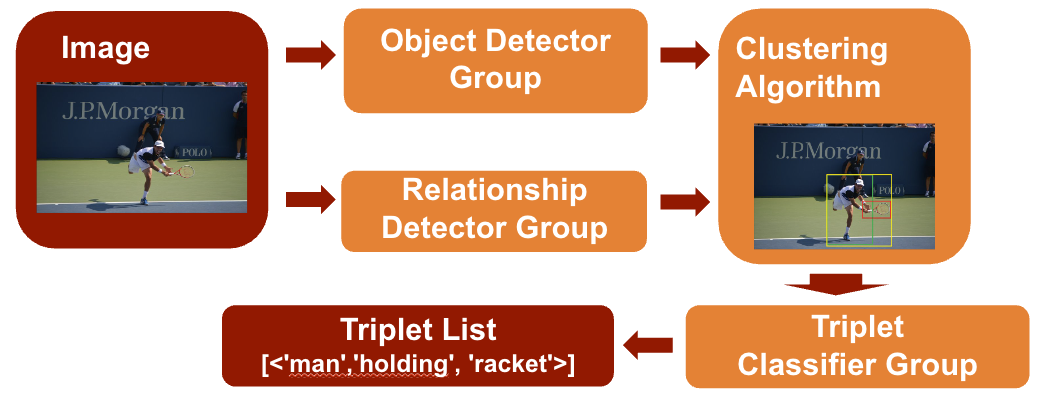
\includegraphics[width=\textwidth]{figures/figure4.png}
  \centering
  \caption{Simple illustration of YOLO-SG's framework.}
\end{figure}
\section{Background and Related Work}
\subsection*{Scene Graph Generation}
Since beginning in 2015 with Johnson et als. work\cite{johnson2015image}, many works have been published improving upon and expanding the scope of SGG\cite{cong2023reltr,desai2021learning,yang2018graph,li2021bipartite,jung2023devil,li2022sgtr,plummer2020revisiting,jin2023fast,lee2018multi,dornadula2019visual,gu2019scene,tripathi2019using,liang2017deep,tang2020unbiased,chiou2021recovering,yan2020pcpl}. Mainstream works often focus on the development of a two-stage scene graph generation approach composed of an object detection stage and a contextual reasoning stage \cite{yang2018graph,jung2023devil}. This two-stage approach the is foundation for most modern SGG methods\cite{yang2018graph,desai2021learning,li2021bipartite,dornadula2019visual,gu2019scene}.
The first stage is often completed using pre-trained detection models\cite{carion2020end}, while contextual reasoning is done using a variety of methods, from convolutional neural networks\cite{yang2018graph} to transformers\cite{cong2023reltr}. To address the quadratic growth of computation relative to object count common in two-stage models, recent works have proposed several one-stage approaches to the problem\cite{cong2023reltr,li2022sgtr}. These models leverage transformer architectures to generate a set of triplets using object information and have been shown to be competitive with two-stage models in terms of performance. However, the large number of parameters required in a transformer architecture also slows down the model inference times, preventing the use of these approaches in real-time applications\cite{cong2023reltr,liang2017deep}.
\paragraph{Long-tailed Distribution Problem}
Several works have been proposed to mitigate the long-tail bias introduced by the data\cite{tang2020unbiased,yu2020cogtree,chiou2021recovering,jin2023fast}. These works can be split into two categories: approaches that used biased training data paired with extra learning techniques or approaches that attempt to remove bias during training.
In the first category, TDE\cite{tang2020unbiased} leverages a causal graph to infer the effect of long-tail bias. CogTree\cite{yu2020cogtree} builds a cognitive structure that distinguishes course-to-fine relationships based on biased predictions. DLFE\cite{chiou2021recovering} uses Dynamic Label Frequency Estimation to recover unbiased probabilities and reduce reporting bias. In the second category, 
The second category of works often approaches the problem by preprocessing training data to remove bias. PCPl\cite{yan2020pcpl} utilizes the correlation between predicate classes to adjust the loss weights. BGNN\cite{li2021bipartite} uses a bi-level data resampling strategy with a confidence-aware bitartite graph to reduce bias. 
One particular work that heavily motivated our approach is the Context Knowledge Network (CKN) proposed by Jin et al. \cite{jin2023fast}, which only uses the object labels and bounds as an input to a multilayer perceptron with the number of possible predicates as the output. Despite the lack of visual information, the authors were still able to achieve competitive high-speed performance with state-of-the-art models, whilst also reducing model bias.
This work motivated our approach with the use of a lightweight MLP similar to CKN, as Jin et al. demonstrated potential in the ability of machine learning models to extract relationship information from non-visual contexts\cite{jin2023fast}. However, our approach differs as we use more than one model, with each model specializing in obtaining confidence scores for only a subset of predicates.
\subsection*{You Only Look Once (YOLO)}
YOLO is a popular object detection model that has been widely used in many computer vision tasks due to its ability to perform single-pass, real-time inferencing. The first version of YOLO proposed by Redmon et al. in 2016 allowed for end-to-end training, as well as object bounding box proposal and object classification in a single forward pass\cite{redmon2016you}.
More importantly, the model was able to achieve this at a rate of 45 frames per second, more than enough for real-time applications. Since then, multiple versions of YOLO have been introduced by various different authors, each of which attempt to improve upon the original whilst following its core design philosophy: open source, end-to-end, and one-shot\cite{terven2023comprehensive}. These newer versions often apply novel techniques to achieve greater overall performance, measured by inference speed, training cost, and inference accuracy\cite{terven2023comprehensive,redmon2017yolo9000,sohan2024review}, 
For our framework, we chose to use the YOLOv11 model due to its higher inference speed compared to YOLOv8 due to the lower number of trained parameters\cite{ultralytics11}. However, it is still possible that performance could be improved using an older version, but this will be left as potential future work.

\section{Framework Design}
 YOLO-SG consists of four main components: an object detection group, a predicate detection group, a clustering stage, and a triplet matching group. The object and predicate detection groups are composed of two sets of YOLOv11 models\cite{redmon2016you}. 
The first set is trained to detect and label objects, while the second set is trained to detect and label predicates. We then split the training data such that every model is provided with a data points consisting only of a subset of predicates that form a balanced dataset relative to the original dataset. By doing so, we obtain multiple unbiased relationship detection models that bound and label their own set of predicate classes instead of a single heavily biased model that predicts all predicate classes at once.
The predicate inference module takes the output of the first stage and obtains a list of objects for each predicate using a simple clustering algorithm.
It then passes every possible pair of objects in this list through a lightweight multilayer perceptron which is trained on the same subset of predicate classes. This then returns confidence scores for that subset of predicates. We then return the triplet with the highest confidence score of the detected predicate as the final output. Since we only use the object labels and positions as inputs as opposed to visual features, we can significantly reduce the number of trained parameters compared to methods that rely on convolutional layers or transformer architectures. 

\paragraph{Example} Suppose we have an image containing a man holding a tennis racket. The 'man' and 'racket' would be bounded and labelled by the object detection group, while the 'holding' relationship would be bounded and labelled by the predicate detection group. The clustering stage would then find all objects, including the man and the racket, that are within the bounds of the 'holding' predicate. The triplet matching group would then pass every possible pair of objects in this list through a lightweight multilayer perceptron trained on the 'holding' predicate class and several other classes. The triplet with the highest confidence score for the 'holding' predicate would then be returned as the final output.

$$
|\text{predicate classes}| = \frac{|\text{triplets of most frequent class}|}{|\text{triplets of least frequent class}|} \leq \text{threshold}
$$
\paragraph{Preprocessing}
Since we need the neural network to interpret words and letters meaningfully, we first convert object and and predicate labels into vectors using GLOVE\cite{pennington2014glove}, a word-to-vector library commonly used by other works on SGG tasks\cite{lee2018multi}. 

To treat predicates as objects, we assign each annotated predicate to a bounding box that encapsulates both the subject and object bounding boxes. For example, given a pair of objects $A,B \in \mathbb{R}^2$ with predicate $r$ in Visual Genome 1.2, we create a new bounding box $R$ that minimally encloses both $A$ and $B$. such that 
Our dataset are separated into wo
In order to represent relationships and objects rather than edges between objects, we must add a corresponding predicate bounding box for each relationship triplet. We define the predicate bounding box $R$ as the minimal bounding box that encapsulates both the subject and object bounding boxes. Given a pair of objects $A,B$ bounding positions $(x_1,y_1,x_2,y_2)$ where $x_1 < x_2, y_1 < y_2$ and a predicate $r$, we define the predicate bounding box $R$ as
$$
R = (\min(A[x_1],B[x_1]),\min(A[y_1],B[y_1]), \max(A[x_2],B[x_2], \max(A[y_2],B[y_2]))
$$
This ensures that each predicate is represented as a single entity in the image which encompasses the subject and object. For example, given a subject with bounding box $A=[100,100,200,200]$ and an object with box $B=[40,140,140,240]$, the bounds for a predicate would be $R=[40,100,200,240]$.
We use the original scene graph annotations to produce a secondary dataset of predicate bounding boxes, each labeled with its corresponding predicate. We now have two datasets which are composed of the same images but different bounding boxes and labels: one has the bounds and labels for objects, while the other has the bounds and labels of predicates. 

\paragraph{Data Splitting}
We split the dataset as follows. We first sort the predicates found in the dataset by the number of instances associated with each predicate. Next, we separate a number of predicates into their own subset. We determine how many predicates to place into the set by calculating the ratio between the number of a instances containing the most frequently occuring predicate with the number of instances containing the least frequently occuring predicate. It follows that the larger the resulting number, the more unbalanced the dataset. For every subset, we select the largest number of predicates ordered by frequency such that the ratio does not exceed a chosen threshold. 

\paragraph{Object Detection}
Our proposed framework, YOLO-SG, decouples the process of object and predicate detection by framing both as object detection tasks. Rather than inferring predicates between every pair of detected objects in a computationally expensive second stage, we directly detect "predicate entities" in parallel alongside object detection. By modeling predicates as distinct objects, we leverage YOLOv11\cite{ultralytics11} for both object and predicate recognition. 
\begin{figure}
    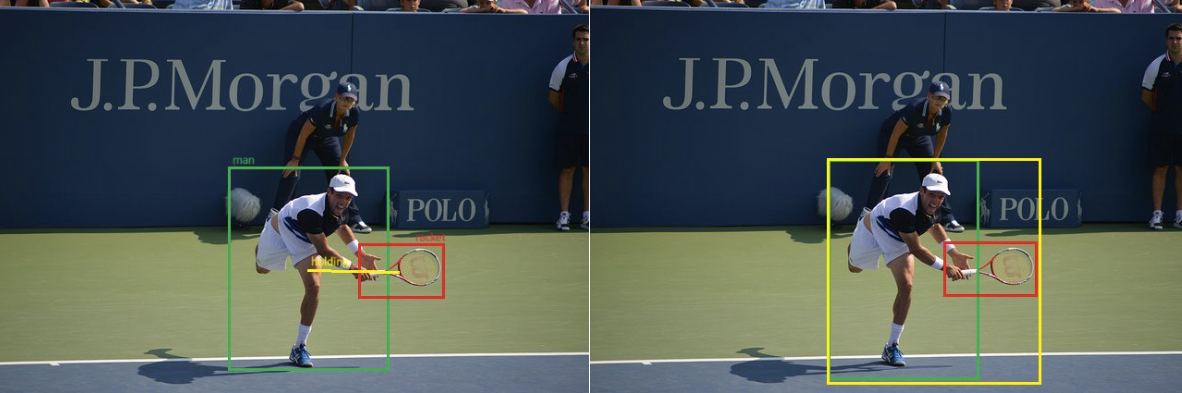
\includegraphics[width=\textwidth]{figures/figure1.png}
  \centering
  \caption{Example of how a predicate bounding box is determined. Given a man holding a racket, the predicate bounding box for 'holding' bounds both the man and the racket.}
\end{figure}

\paragraph{Clustering Algorithm}
We chose to use an Intersection-Over-Union (IoU) based clustering algorithm to associate detected objects with their corresponding predicates due to its simplicity and low time complexity. Given $n$ objects, the algorithm has a worst-case complexity of $O(n \log n)$. For each predicate entity detected, we calculate the IoU of objects that overlap with the predicate bounds, grouping all objects that have an IOU larger than 0.5 with the predicate bounding box. Due to time constraints, we did not perform experiments to determine the optimal IOU threshold, and this is left as potential future work.

\paragraph{Triplet Matching}
After obtaining a list of objects for each predicate, we need to determine which object pair is most likely to be associated with the predicate. We use a lightweight multilayer perceptron (MLP) to score the plausibility of each object pair. The MLP has a total of <!!!> GLOVE vectors corresponding to the objects, the bou  has three fully connected layers with ReLU activation functions. The is trained on the same subset of predicate classes as the predicate detection model. For each predicate detection, we run the MLP once for every potential object pair that can be formed by objects in the list, selecting the triplet which returns the highest confidence score for the predicate class label.

\section{Experiment}
\subsection{Dataset}
We use the Visual Genome (VG) 1.2 dataset, a dataset widely used for SGG benchmarking that is composed of more than 108 thousand images and 2.3 million relationship predicates \cite{krishna2017visual} as our training and test set.
note that the Visual Genome dataset contains a large number of object and predicate labels which are semantically equivalent to one another (for example, 'under' and 'below'). In a recent release, the maintainers of the dataset has provided us with a collection of synonym sets that group similar objects and predicates into the same class, with one term assigned by group. After converting all synonymous terms to their respective group representative term, we remove objects which rarely appear along with any associated triplets. 
After preprocessing, we split VG into training and test sets in the manner proposed by \cite{xu2017scene} as it is most commonly used by similar works\cite{cong2023reltr,yang2018graph}. We end up with a training set containing 73k images and a test set containing 35k images. 

\subsection{Training}
Since the data used in every module is independent of the performance of other modules, we train every module in parallel. 
We train both the object detection and predicate detection models using the YOLOv11 architecture on the same images. However, we only train the object dection models on the bounding box class labels provided by the dataset. For the predicate detection model, we use the predicate bounding boxes that we created during preprocessing. During training, We set the learning rate to 0.0001, the batch size to 32, and the maximum epochs to 300. We train the YOLO models on 5 NVIDIA 4090Ti graphics cards, with training taking 25 hours to complete. The multi-layer perceptrons used for triplet matching are trained using the information of the triplets for the predicate classes that the model is specialized in classifying. Since the number of trained parameters is significantly lower, training the MLPs on a single NVIDIA 3060 graphics card takes only 2 hours.

\begin{figure}
    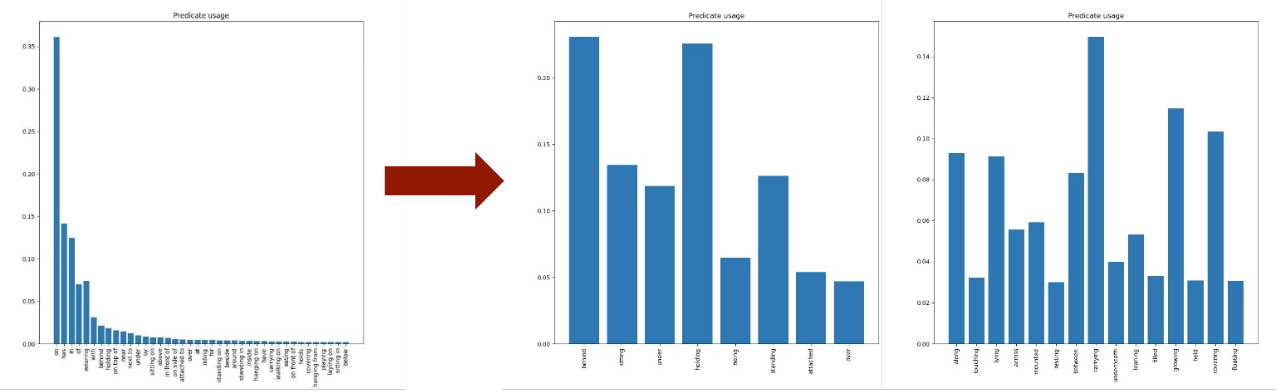
\includegraphics[width=\textwidth]{figures/figure2.png}
  \centering
  \caption{Illustration of dataset splitting results. The left histogram shows the data distribution of the top 50 most frequent predicate classes, while the two right histograms show the distributions of two predicate subsets after splitting. In this example, the threshold ratio is set to 5.}
\end{figure}

\begin{figure}
    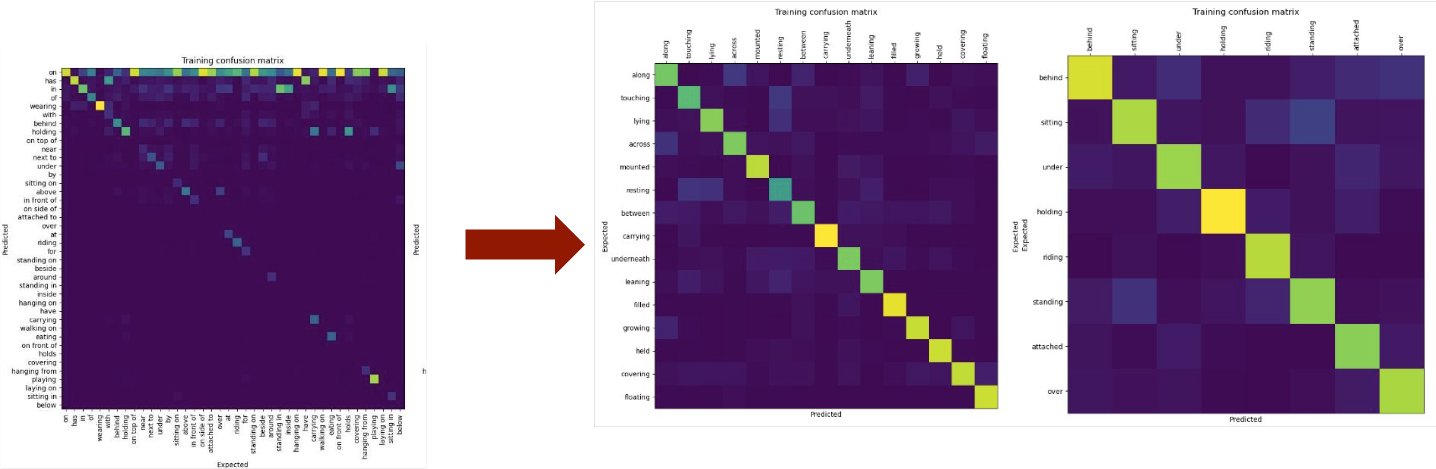
\includegraphics[width=\textwidth]{figures/figure3.png}
  \centering
  \caption{Predicate classification results before and after data splitting. The left image shows the confusion matrix on a sample of predicates for a YOLO model that is given the original dataset in its entirety, while the right matrices demonstrate the results of several models with the same architecture trained on subsets of the sample.}
\end{figure}
\subsection{Evaluation Metrics}
The task of scene graph generation can be divided into several subtasks, each with varying levels of difficulty. Predicate classification (PredCLS)\cite{cong2023reltr,jin2023fast,dornadula2019visual} predicts predicates given the subject and object labels and bounds. Scene graph classification (SGCLS)\cite{cong2023reltr,dornadula2019visual} predicts the triplet labels given the bounding boxes. Scene graph detection (SGDET)\cite{cong2023reltr}, also referred to simply as Scene graph generation (SGGen)\cite{jin2023fast,dornadula2019visual}, predicts the labels and bounding boxes of all three elements.
Due to time constraints, we only evaluate the model on the SGGen. This is already sufficient, as SGGen is the most difficult task and the one that we are chiefly concerned about. We follow the common standard set by previous works\cite{cong2023reltr, yang2018graph, li2022sgtr, jin2023fast, yan2020pcpl} and adopt the evaluation metric mean recall@K (mR@K). Given a single image, Recall@$k$ is defined as the fraction of ground truth triplets which can be found in the top $k$ triplet predictions. Two triplets are considered equivalent when all three elements (subject, predicate, and object) have been labelled correctly and both object and subject bounding boxes have IoU > 0.5 compared to the ground truth bounding boxes. We compute the mean recall at K=50 and K=100 for our experiments. 

\subsection{Results}
\begin{table}[]
\caption{Comparison of YOLO-SG with other state-of-the-art models on the Visual Genome 1.2 dataset. the best results in each category are bolded.}
    \centering
\begin{tabular}{cccc}
\hline
\multirow{2}{*}{Method} & \multicolumn{2}{c|}{SGGen} & \multirow{2}{*}{FPS}  \\
                        & mR@50       & mR@100       &      \\ \hline
RelTr                   & 10.8        & 12.6         & 16.3 \\
SGTR                    & 15.8        & \textbf{20.1}         & 3.8  \\
C-SGG                   & 14.8        & 17.1         & 33.5 \\
G-RCNN                  & 6.1        & 7.2         & -    \\
BGNN                    & 10.7        & 12.6         & 2.9 \\
PCPL                    & 10.4        & 14.4         & -    \\
MOTIFS                  & 5.7         & -            & 6.6  \\ \hline
\textbf{YOLO-SG} (ours)                 & \textbf{17.5}        & 17.5            & \textbf{43.3} \\ \hline
\end{tabular}
\end{table}

Our model achieves a mean recall of 17.5 at K=50 and K=100, outperforming all other models in the comparison. We also achieve the highest inference speed of 43.3 frames per second, which is significantly higher than other models, clearly demonstrating the effectiveness of our approach. Compared to C-SGG\cite{jin2023fast}, which inspired our MLP triplet matching stage, we achieve both higher recall and higher inference speed. This is likely due to the fact that our model is able to leverage the high accuracy of YOLOv11 in object detection, an important component of the scene graph generation task. 
\paragraph{Threats to Validity}
Despite our very promising results, there are many additional changes and further experiments that need to be made in order for the validity of our results to be strong, as there are multiple reasons besides the design of our architecture for the higher performance.
Since we used the recently-released YOLOv11 architecture, it is possible that the higher performance is due to the improvements made in the architecture itself, as older models that we compare against use older, less optimized architectures. Additionally, we only evaluate our model on the SGGen task, and it is possible that results on the PredCLS and SGCLS tasks can reveal flaws or further potential improvements in the design of YOLO-SG.
Also note that for all other models that we compare YOLO-SG, recall consistently increases with a higher $K$, yet does not increase for YOLO-SG. We believe that this is due to a flaw in our implementation, as the number of predictions must be equal to the number of relationship predicates.
Hence, while other models will make multiple predictions with the same predicate but multiple different object-subjects, our will only make one, hence limiting the effect that increasing K has on performance. We can alleviate this problem by including multiple predictions for the same predicate, ranked by confidence score. 


\section{Conclusions}
In this work, we propose YOLO-SG, a novel scene graph generation framework that redefines the task of SGG by treating relationships as objects. By using multiple detection models in parallel, We to reduce the long-tail bias caused by the data distribution while at the same time achieving competitive performance and speed with state-of-the-art models. However, there is still a signficant amount of future work required to solidify the validity of the study. We still need to conduct an ablation study to determine the impacts of YOLOv11 on the model's performance by changing to older versions. We also need to conduct exploratory experiments to fine-tune the model parameters, notably the IoU threshold for clustering and the split factor. Finally, we need to resolve some minor flaws that were discovered after evaluation, such as the limiting of predictions to one per predicate found. We believe that with these changes, YOLO-SG can become a powerful tool that offers a new perspective on  scene graph generation.

\newpage
\bibliography{citations}
\end{document}



